\documentclass[12pt,titlepage]{article}
\usepackage[margin=1.25in]{geometry}
\usepackage{graphicx,amsmath,minted}
\usepackage{pgf-umlcd}

%% Variables definition
\newcommand{\vSubject}{Data Structure and Algorithm Practicum}
\newcommand{\vSubtitle}{Queue}
\newcommand{\vName}{Dicha Zelianivan Arkana}
\newcommand{\vNIM}{2241720002}
\newcommand{\vClass}{1i}
\newcommand{\vDepartment}{Information Technology}
\newcommand{\vStudyProgram}{D4 Informatics Engineering}

%% [START] Tikz related stuff
\usepackage{tikz}
\usetikzlibrary{svg.path,calc,shapes.geometric,shapes.misc}
\tikzstyle{terminator} = [rectangle, draw, text centered, rounded corners = 1em, minimum height=2em]
\tikzstyle{preparation} = [chamfered rectangle, chamfered rectangle sep=0.75em, draw, text centered, minimum height = 2em]
\tikzstyle{process} = [rectangle, draw, text centered, minimum height=2em]
\tikzstyle{decision} = [diamond, aspect=2, draw, text centered, minimum height=2em]
\tikzstyle{data}=[trapezium, draw, text centered, trapezium left angle=60, trapezium right angle=120, minimum height=2em]
\tikzstyle{connector} = [line width=0.25mm,->]
%% [END] Tikz related stuff

%% [START] Fancy header related stuff
\usepackage{fancyhdr}
\pagestyle{fancy}
\setlength{\headheight}{15pt} % compensate fancyhdr style
\fancyhead{}
\fancyfoot{}
\fancyfoot[L]{\thepage}
\fancyfoot[R]{\textit{\vSubject - \vSubtitle}}
\renewcommand{\footrulewidth}{0.4pt}% default is 0pt, overline for footer
%% [END] Fancy header related stuff

%% [START] Custom tabular command related stuff
\usepackage{tabularx}
\newcommand{\details}[2]{
    #1 & #2  \\
}
%% [END] Custom tabular command related stuff

%% [START] Figure related stuff
\newcommand{\image}[3][1]{
    \begin{figure}[h]
        \centering
        \includegraphics[#1]{#2}
        \caption{#3}
        \label{#3}
    \end{figure}
}
%% [END] Figure related stuff

\begin{document}
\begin{titlepage}
    \centering
    \vfill
    {\bfseries\LARGE
        \vSubject\\
        \vskip0.25cm
        \vSubtitle
    }
    \vfill
    
\includegraphics[width=6cm]{images/polinema-logo.png}
    \vfill
    {
        \textbf{Name}\\
        \vName\\
        \vskip0.5cm
        \textbf{NIM}\\
        \vNIM\\
        \vskip0.5cm
        \textbf{Class}\\
        \vClass\\
        \vskip0.5cm
        \textbf{Department}\\
        \vDepartment\\
        \vskip0.5cm
        \textbf{Study Program}\\
        \vStudyProgram
    }
\end{titlepage}

\section*{Lab Activities \#1}
\subsection*{Questions}
\begin{enumerate}
    \item {
        In method \texttt{create()}, why is the front and rear attribute has initial value with 1 and not 0?

        Because 0 marks the first element while -1 marks that the queue hasn't been filled with any element
    }
    \item {
        In method \texttt{enqueue()}, please explain the usage of this following code

        \begin{minted}[autogobble,fontsize=\small]{java}
            if (rear == max - 1) {
                rear = 0;
            }
        \end{minted}

        This is used to cycle the rear position of the queue. If the rear is at the last position,
        then we should back to the beginning of the array, otherwise we'll get an array index out of bound exception
    }
    \item {
        Observe \texttt{dequeue()} method, which line of code indicates that the data is removed in the first
        position of the queue?

        \begin{minted}[autogobble,fontsize=\small]{java}
            data = Q[front];
            size--;
            if (isEmpty()) {
                front = rear = -1;
            } else {
                if (front == max - 1) {
                    front = 0;
                } else {
                    front++;
                }
            }
        \end{minted}

        This part indicates that we take the first data in the queue by doing \texttt{data = Q[front]}
        and then resetting the front position to the next item in the queue, effectively removing access to the first
        element that we remove
    }
    \item {
        In \texttt{dequeue()} method, explain the usage of these codes!
        
        \begin{minted}[autogobble,fontsize=\small]{java}
            if (front == max - 1) {
                front = 0;
            }
        \end{minted}

        Same as in the \texttt{enqueue()} method, this is used to reset the position of the front element of the queue
        when it reaches the end of the array so that we don't get index out of bound exception.
    }
    \item {
        In method \texttt{print()}, why the loop process has \texttt{int i = 0} instead of \texttt{int i = front}?

        There is no \texttt{int i = 0} to begin with. The codes uses \texttt{int i = front} so this question is invalid.
        However, the explanation is that we use \texttt{i = front} because the beginning of the queue isn't always at the start of the array.
        If we would use \texttt{i = 0}, we might start looping from the middle of the queue.
    }
    \item {
        In method \texttt{print()}, please explain why we insert this code in our program?
        
        \begin{minted}[autogobble,fontsize=\small]{java}
            i = (i + 1) % max;
        \end{minted}

        This is used to go back at the start of the array when we reach the end of it. Since the queue is circular to the array,
        we need to modulus the index with the maximum amount of the queue, which makes it reset to the 
    }
\end{enumerate}

\section*{Lab Activities \#2}
\subsection*{Questions}
\begin{enumerate}
    \item {
        In \texttt{Queue} class, what's the function of this program code in method \texttt{dequeue()} ?

        \begin{minted}[autogobble,fontsize=\small]{java}
            Passenger data = new Passenger("", "", "", 0, 0);
        \end{minted}

        It's used to fill in the initial data when we haven't found the data on the queue yet. We construct
        a dummy empty passenger object since we're still unsure if the queue contains any data or not.
    }
    \item {
        In previous number, if the program code changed to

        \begin{minted}[autogobble,fontsize=\small]{java}
            Passenger data = new Passenger();
        \end{minted}

        What will happen?

        It will throw an error because the constructor requires 5 arguments and because we define the constructor with parameters,
        Java won't create an implicit parameter-less constructor.
    }
    \item {
        Show the program code used for displaying the data retrieved / removed from the queue!

        \pagebreak

        It's in the second branch of the switch case as shown below:

        \begin{minted}[autogobble,fontsize=\small]{java}
            Passenger data = queuePassenger.dequeue();
            if (/* removed for brevity, long condition empty string check */) {
                System.out.println(/* the detail of the passenger concatenated to a string */)
            }
        \end{minted}
    }
    \item {
        Modify the program by adding a method named \texttt{peekRear()} in Queue class to check the
        last position within the queue. Add a menu for the user to perform and explore your program as well

        \begin{minted}[autogobble,fontsize=\small]{java}
            public void peekRear() {
                if (!isEmpty()) {
                    System.out.println("The last element : " +
                            Q[rear].name + " " +
                            Q[rear].cityOrigin + " " +
                            Q[rear].cityDestination + " " +
                            Q[rear].ticketAmount + " " +
                            Q[rear].price
                    );
                } else {
                    System.out.println("Queue is still empty");
                }
            }
        \end{minted}

        We can add the menu enty as such:
        
        \begin{minted}[autogobble,fontsize=\small]{java}
            // rest of the code above
            System.out.println("3. Print");
            System.out.println("4. Peek");
            System.out.println("5. Peek Rear"); // the new menu
            System.out.println("6. Clear");
            System.out.println("=======================");
            // rest of the code below

            // rest of the code above
            case 4:
                Q.peek();
                break;
            case 5: // new addition to peek the rear of the queue
                Q.peekRear();
                break;
            case 6:
                Q.clear();
                break;
            // rest of the code below
        \end{minted}
    }
    \item {
        Ensure that the \texttt{peekRear()} function can be executed inside the program

        \begin{figure}[h]
            \centering
            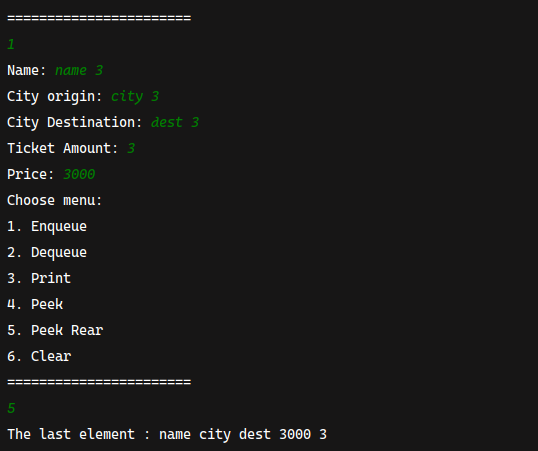
\includegraphics[width=.8\textwidth]{./images/peek_rear_output.png}
        \end{figure}
    }
\end{enumerate}

\subsection*{Assignments}
\begin{enumerate}
    \item {
        Add these 2 methods in \texttt{Queue} class in $1^{st}$ practicum

        The question is ambiguous as there are no methods listed to add to the program.
        So, I'm stuck.
    }
    \item {
        Make a queue program for students when they need the signs for their KRS by the DPA.
        If the student is in the queue, they will be required to fill in some information as follows:

        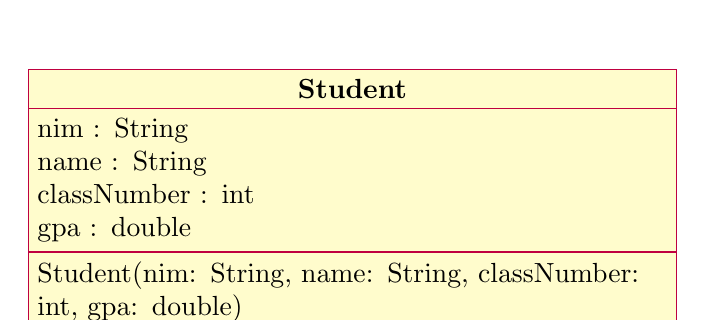
\begin{tikzpicture}
            \begin{class}[text width=8cm]{Student}{0,0}
                \attribute{nim : String}
                \attribute{name : String}
                \attribute{classNumber : int}
                \attribute{gpa : double}
                \operation{Student(nim: String, name: String, classNumber: int, gpa: double)}
            \end{class}
        \end{tikzpicture}

        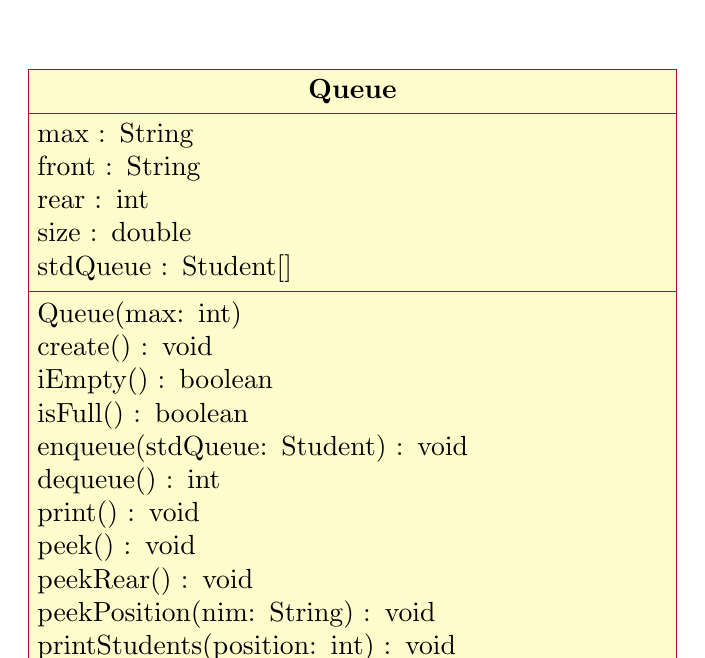
\begin{tikzpicture}
            \begin{class}[text width=8cm]{Queue}{0,0}
                \attribute{max : String}
                \attribute{front : String}
                \attribute{rear : int}
                \attribute{size : double}
                \attribute{stdQueue : Student[]}
                \operation{Queue(max: int)}
                \operation{create() : void}
                \operation{iEmpty() : boolean}
                \operation{isFull() : boolean}
                \operation{enqueue(stdQueue: Student) : void}
                \operation{dequeue() : int}
                \operation{print() : void}
                \operation{peek() : void}
                \operation{peekRear() : void}
                \operation{peekPosition(nim: String) : void}
                \operation{printStudents(position: int) : void}
            \end{class}
        \end{tikzpicture}

        Notes:
        \begin{itemize}
            \item {
                The implementation of 
                \begin{itemize}
                    \item \texttt{create()}
                    \item \texttt{isEmpty()} 
                    \item \texttt{isFull()}
                    \item \texttt{enqueue()}
                    \item \texttt{dequeue()}
                    \item and \texttt{print()}
                \end{itemize}
                functions are similar with what we've build in practicum
            }
            \item {
                \texttt{peek()} method is used for displaying students data in the first queue
            }
            \item {
                \texttt{peekRead()} method is used for displaying students data in the last queue
            }
            \item {
                \texttt{peekPosition()} method is used for displaying students data in the queue by their NIM
            }
            \item {
                \texttt{printStudents()} method is used for displaying a student data in specified position in a queue
            }

            \pagebreak

            \large{\textbf{Code}}
            \begin{itemize}
                \item {
                    \textbf{Student.java}

                    \begin{minted}[autogobble,fontsize=\footnotesize]{java}
                        public class Student {
                            String nim;
                            String name;
                            int classNumber;
                            double gpa;

                            public Student(String nim, String name, int classNumber, double gpa) {
                                this.nim = nim;
                                this.name = name;
                                this.classNumber = classNumber;
                                this.gpa = gpa;
                            }
                        }
                    \end{minted}
                }
                \item {
                    \textbf{StudentQueue.java}

                    \begin{minted}[autogobble,fontsize=\footnotesize]{java}
                        public class StudentQueue {
                            int max;
                            int size;
                            int front;
                            int rear;
                            Student[] Q;

                            public StudentQueue(int n) {
                                max = n;
                                create();
                            }

                            public void create() {
                                Q = new Student[max];
                                size = 0;
                                front = rear = -1;
                            }

                            public boolean isEmpty() {
                                return size == 0;
                            }

                            public boolean isFull() {
                                return size == max;
                            }

                            public void peek() {
                                if (!isEmpty()) {
                                    System.out.println(
                                        "The first element : " + 
                                        Q[front].nim + " " + 
                                        Q[front].name + " " + 
                                        Q[front].classNumber + " " + 
                                        Q[front].gpa
                                    );
                                } else {
                                    System.out.println("Queue is still empty");
                                }
                            }

                            public void peekRear() {
                                if (!isEmpty()) {
                                    System.out.println("The last element : " + 
                                        Q[rear].nim + " " + 
                                        Q[rear].name + " " + 
                                        Q[rear].classNumber + " " + 
                                        Q[rear].gpa
                                    );
                                } else {
                                    System.out.println("Queue is still empty");
                                }
                            }

                            public void print() {
                                if (isEmpty()) {
                                    System.out.println("Queue is still empty");
                                    return;
                                }

                                int i = front;
                                while (i != rear) {
                                    System.out.println(
                                        Q[i].nim + " " +
                                        Q[i].name + " " +
                                        Q[i].classNumber + " " + 
                                        Q[i].gpa
                                    );
                                    i = (i + 1) % max;
                                }
                                System.out.println(
                                    Q[front].nim + " " +
                                    Q[front].name + " " +
                                    Q[front].classNumber + " " +
                                    Q[front].gpa
                                );
                                System.out.println("Element amount : " + size);
                            }

                            public void clear() {
                                if (!isEmpty()) {
                                    front = rear = -1;
                                    size = 0;
                                    System.out.println("Queue has been cleared successfully");
                                } else {
                                    System.out.println("Queue is still empty");
                                }
                            }

                            public void enqueue(Student data) {
                                if (isFull()) {
                                    System.out.println("Queue is already full");
                                    return;
                                }

                                if (isEmpty()) {
                                    front = rear = 0;
                                } else {
                                    rear = rear == max - 1 ? 0 : rear + 1;
                                }

                                Q[rear] = data;
                                size++;
                            }

                            public Student dequeue() {
                                Student data = new Student("", "", 0, 0);
                                if (isEmpty()) {
                                    System.out.println("Queue is still empty");
                                } else {
                                    data = Q[front];
                                    size--;
                                    if (isEmpty()) {
                                        front = rear = -1;
                                    } else {
                                        if (front == max - 1) {
                                            front = 0;
                                        } else {
                                            front++;
                                        }
                                    }
                                }
                                return data;
                            }

                            void peekPosition(String nim) {
                                Student student = null;
                                for (Student queuedStudent : Q) {
                                    if (queuedStudent == null) continue;
                                    if (nim.equals(queuedStudent.nim)) {
                                        student = queuedStudent;
                                        break;
                                    }
                                }

                                if (student != null) {
                                    System.out.println(
                                        "Selected Student : " +
                                        student.name + " " +
                                        student.nim + " " +
                                        student.classNumber + " " +
                                        student.gpa
                                    );
                                    return;
                                }

                                System.out.println("The Inputted NIM isn't available");
                            }

                            void printStudents(int pos) {
                                int index = (pos + front) % max;
                                if (Q[index] == null) {
                                    System.out.println("There is no Student at that queue");
                                    return;
                                }
                                System.out.println("Selected Student : " +
                                    Q[index].name + " " +
                                    Q[index].nim + " " +
                                    Q[index].classNumber + " " +
                                    Q[index].gpa
                                );
                            }
                    \end{minted}
                }
            \end{itemize}
        \end{itemize}
    }
\end{enumerate}

\end{document}

